\chapter{Sensitivity studies: production of $\chinopm$ and $\nino$}
    \label{sec:CharginoNeutralinoProduction}

In this appendix, sensitivity studies are carried out for models involving squark-neutralino, chargino-neutralino, and neutralino-neutralino direct productions.
Monte Carlo samples for these models have been produced using \madgraph{}, interfaced with \pythia{} to model the parton showering and hadronization.
The monojet analysis is expected to have low sensitivity to these models, and for this reason, the reconstruction of the physics objects is done with \delphes{}~\cite{Ovyn:2009tx}.
\delphes{} provides a very simple parametrization of the ATLAS detector acceptances, efficiencies and resolution, but does not model the trigger efficiency, the charged fraction and the electromagnetic fraction in the calorimeter.
Altogether, this results into an about 10\% to 20\% difference between the signal acceptance predicted by \delphes{} and the ATLAS simulation.

The sensitivity studies, closely follow the strategy used in Chapter~\ref{sec:GravitinoProduction} for the light gravitino production in GMSB scenarios.
The ratio $\sigma(\text{SUSY})/$ $\sigma(\text{obs})$ is computed, where $\sigma (SUSY)$ is the expected fiducial cross section for the signal model, and $\sigma (obs)$ are the observed model independent limits of the monojet analysis, listed in Table \ref{tab:modelIndependent}.
Models for which $\sigma (SUSY) / \sigma (obs) > 1$ are excluded at 95\% CL.


\section{Squark-neutralino production}
    \label{subsec:SquarkNeutralinoProduction}

The study of the associated production of a scalar quark and a neutralino, $\squarkneutralino$ (see Figure \ref{fig:DiagramsElectroweakProduction} left), provides information on the coupling to the $\ninoone$ as a DM candidate.
Samples with squark mass ranges between $\unit[100]{GeV}$ and $\unit[1000]{GeV}$ have been generated for neutralino masses between 0~GeV and those values corresponding to a $\Delta m = m_{\squark} - m_{\ninoone} = \unit[3]{GeV}$.
Since the squark, $\squark$, decays into a quark, $q$, and a neutralino, $ \ninoone$, the squark-neutralino production leads to a final state with an energetic jet and $\met$.

Figure \ref{fig:squarkNeutralinoBestRegion} shows the signal region with the best sensitivity (higher $\sigma (SUSY) / \sigma (obs)$ ratio) for the different parameter configurations of this model.
Regions M1, M2, M3 and M4 are found to be optimal for different values of $m_{\squark}$ and $m_{\ninoone}$.

\begin{figure}[!ht]
\begin{center}
\mbox{
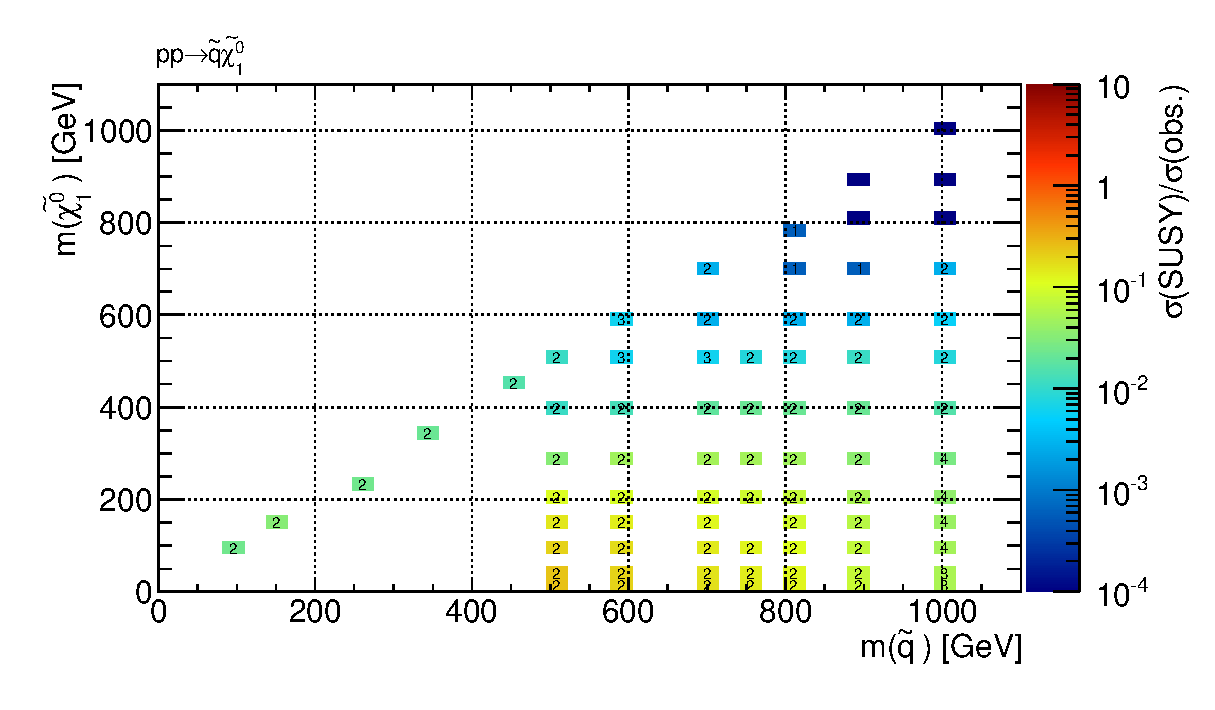
\includegraphics[width=0.995\textwidth]{Interpretations/Figures/sq_neu_best.eps}
}
\end{center}
\caption[Ratio between the expected fiducial cross section for each squark-neutralino model, $\sigma (SUSY)$, and the observed model independent limit.]{Ratio between the expected fiducial cross section for each squark-neutralino model, $\sigma (SUSY)$, and the observed model independent limit, $\sigma (obs)$, in the $m_{\squark}$-$m_{\ninoone}$ plane. The numbers in the boxes correspond to the index of the signal region with the best sensitivity.}
\label{fig:squarkNeutralinoBestRegion}
\end{figure}

The $\sigma (SUSY) / \sigma (obs)$ for the signal region providing the best sensitivity is shown in Figure~\ref{fig:squarkNeutralinoLimits} as a function of $m_{\squark}$, for $\Delta m$ values of 100~GeV and 500~GeV.
The best sensitivity is obtained for $m_{\squark} = \unit[500]{GeV}$ and very small $m_{\ninoone}$.
For this configuration of parameters, an energetic jet from the decay of the squark is produced in association to high $\pt$ neutralinos.

The cross section of the signal is between one and four orders of magnitude smaller than the minimum visible cross section needed to provide any exclusion, in all the parameter space.
Therefore, the possibility of setting limits in this region of the phase space with an early monojet analysis at 13~TeV is practically excluded.

\begin{figure}[!ht]
\begin{center}
\mbox{
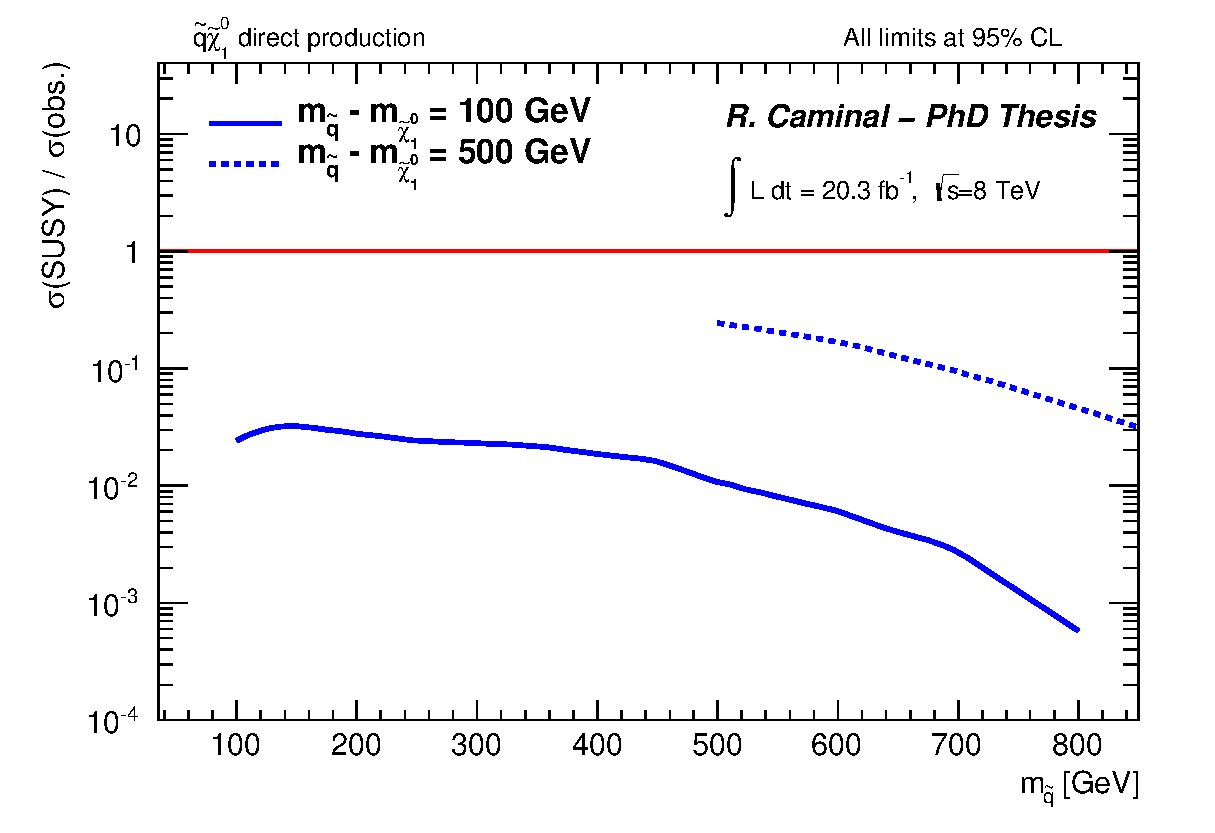
\includegraphics[width=0.795\textwidth]{Interpretations/Figures/sq_neu_limits.eps}
}
\end{center}
\caption[Ratio $\sigma (SUSY) / \sigma (obs)$ as a function of $m_{\squark}$ for different $\Delta m$ values.]{Ratio $\sigma (SUSY) / \sigma (obs)$ as a function of $m_{\squark}$ for $\Delta m = 100,\, 500$~GeV. For each mass point the best signal region giving the best ratio is used.}
\label{fig:squarkNeutralinoLimits}
\end{figure}


\section{Chargino-chargino and neutralino-chargino production}
    \label{subsec:NeutralinoCharginoProduction}

Exclusion limits at the 95\% CL on the direct production of charginos and neutralinos decaying to different final states have been computed by several analyses in ATLAS \cite{Aad:2014nua}, and are summarized in Figure~\ref{fig:SUSYEWSummary}.
In compressed scenarios where $m_{\ninotwo} \leq m_{\ninoone} + m_Z$ and/or $m_{\chinoonepm} \leq m_{\ninoone} + m_{W^{\pm}}$, the gauge bosons are off-shell and produce soft leptons or jets that may not be reconstructed.
After requiring that the system is balanced by an initial-state radiation jet, these models lead to monojet plus high $\met$ final states.

\begin{figure}[!ht]
\begin{center}
\mbox{
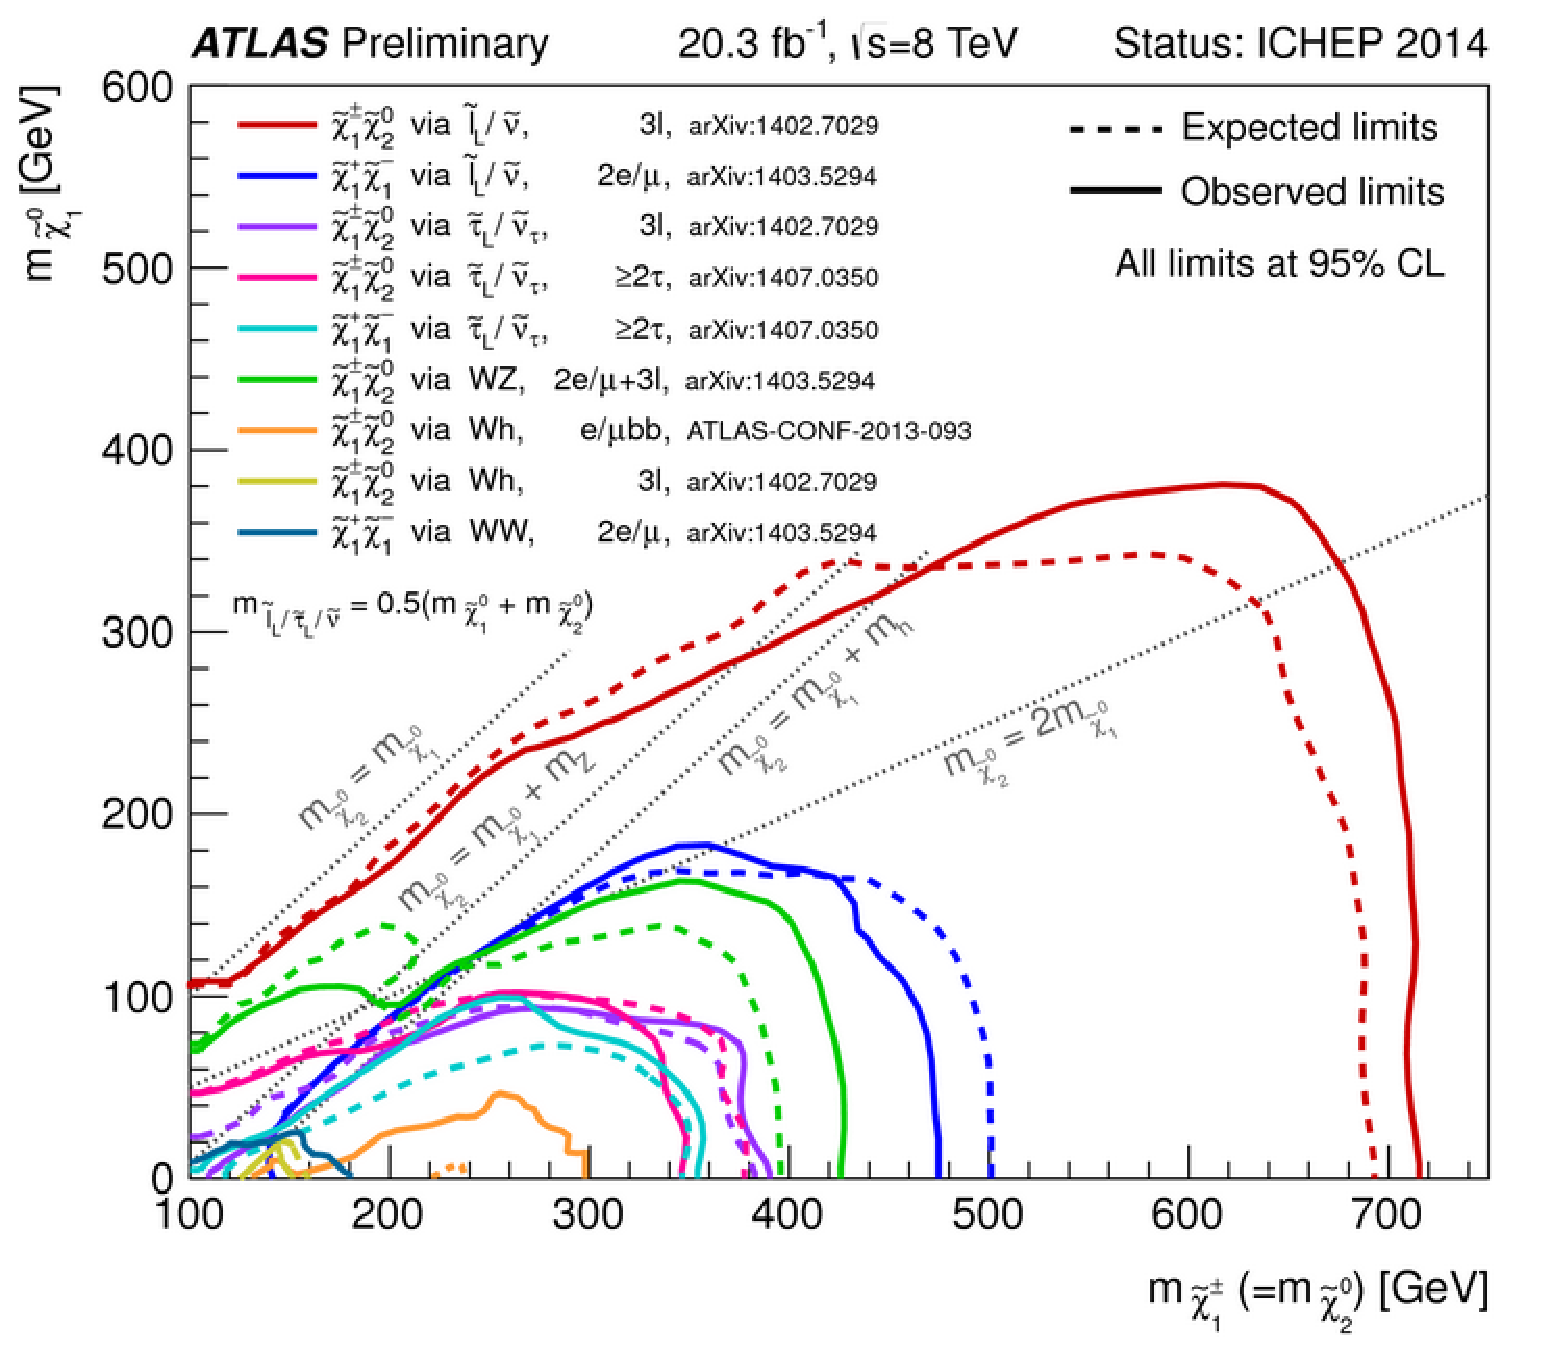
\includegraphics[width=0.795\textwidth]{Interpretations/Figures/ATLAS_SUSY_EWSummary.eps}
}
\end{center}
\caption[Summary of ATLAS searches for electroweak production of charginos and neutralinos.]{Summary of ATLAS searches for electroweak production of charginos and neutralinos on $\unit[20]{fb^{-1}}$ of $\pp$ collision data at $\sqrt{s} = \unit[8]{TeV}$ \protect\cite{Aad:2014nua}. Exclusion limits at $95\%$ CL are shown in the $m_{\chinoonepm} = m_{\ninotwo}$, $m_{\ninoone}$ plane. The dashed and solid lines show the expected and observed limits respectively, including all uncertainties except the theoretical ones affecting the signal cross sections.}
\label{fig:SUSYEWSummary}
\end{figure}

Figure~\ref{fig:NeutralinoNeutralinoBestRegion} shows the ratio $\sigma (SUSY) / \sigma (obs)$ obtained in the most sensitive signal region for the generated samples with different mass configurations.
The best sensitivity is obtained for the selection M2 in the region of the parameter space with small $\Delta m$, and for the selection M1 in models with low $m_{\ninotwo , \chinoonepm}$ and high $\Delta m$.
The value of $\sigma (SUSY) / \sigma (obs)$ as a function of $m_{\ninotwo , \chinoonepm}$ is shown in Figure~\ref{fig:NeutralinoNeutralinoLimits} for $\Delta m = \unit[5,\, 25,\, 50]{GeV}$. 
The best sensitivity is obtained for low $m_{\ninotwo , \chinoonepm}$ and the $\Delta m = \unit[5]{GeV}$.
The monojet analysis is not sensitive enough to exclude any region of the parameter space under consideration, but the compressed configurations with low values of $m_{\ninotwo , \chinoonepm}$ are only a factor 2 below the threshold sensitivity.
These configurations might become important in future interpretations of the monojet analysis at 13~TeV.

\begin{figure}[!ht]
\begin{center}
\mbox{
\includegraphics[width=0.995\textwidth]{Interpretations/Figures/NN-NC_grid.eps}
}
\end{center}
\caption[Ratio between the expected fiducial cross section of $\ninotwo \chinoonepm$, $\chinoonepm \chinoonemp$ and the monojet observed model independent limit in the $m_{\ninotwo , \chinoonepm}$-$m_{\ninoone}$ plane.]{Ratio between the expected fiducial cross section of $\ninotwo \chinoonepm$, $\chinoonepm \chinoonemp$ ($\sigma (SUSY)$) and the monojet observed model independent limit ($\sigma (obs)$) in the $m_{\ninotwo , \chinoonepm}$-$m_{\ninoone}$ plane. The numbers on the boxes correspond to the index of the signal region with the best sensitivity.}
\label{fig:NeutralinoNeutralinoBestRegion}
\end{figure}

\begin{figure}[!ht]
\begin{center}
\mbox{
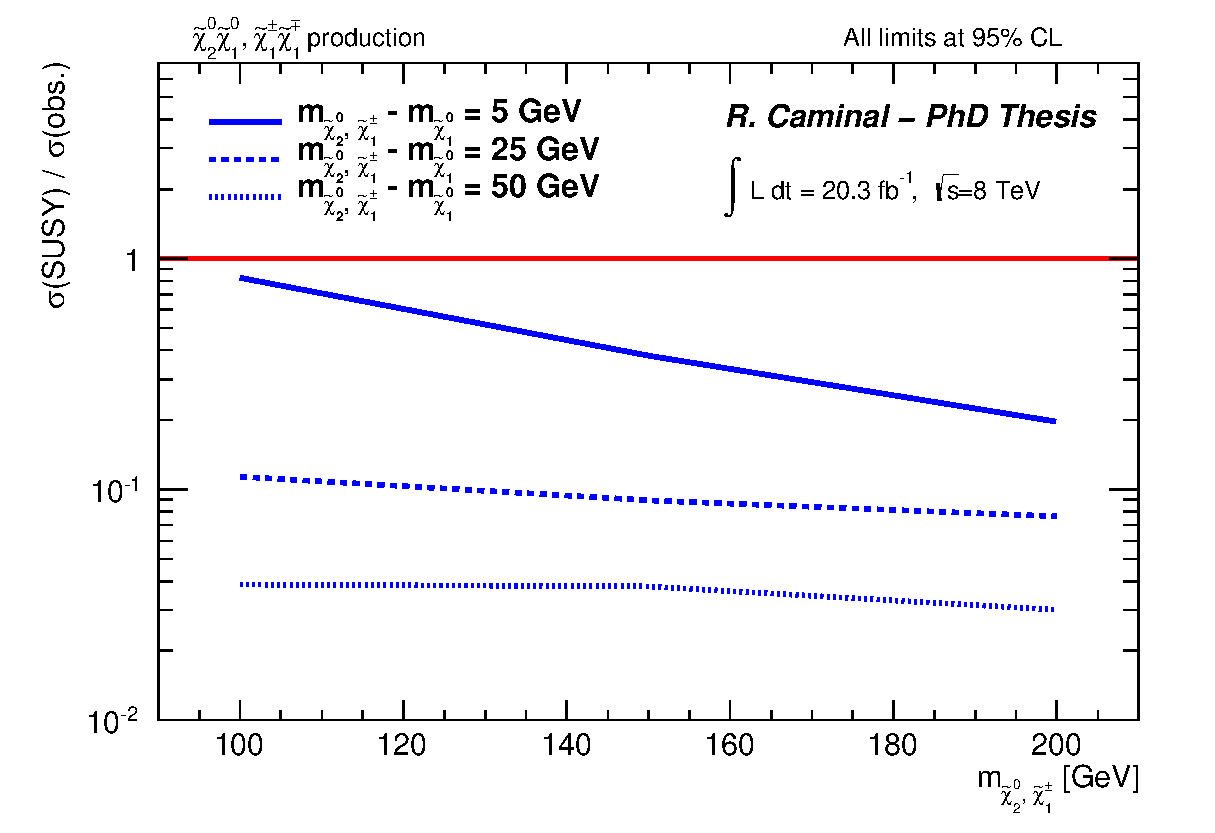
\includegraphics[width=0.795\textwidth]{Interpretations/Figures/NN-NC_best.eps}
}
\end{center}
\caption[Ratio $\sigma (SUSY) / \sigma (obs)$ as a function of $m_{\ninotwo , \chinoonepm}$ for $\Delta m = 5, 25, 50$~GeV.]{Ratio $\sigma (SUSY) / \sigma (obs)$ as a function of $m_{\ninotwo , \chinoonepm}$ for $\Delta m = \unit[5,\, 25,\, 50]{GeV}$.}
\label{fig:NeutralinoNeutralinoLimits}
\end{figure}
